\documentclass{beamer}
\usepackage[utf8]{inputenc}
\usepackage{pdfpages}
\usepackage{graphicx}
\usepackage{listings}
\usepackage{color}

\definecolor{mygreen}{rgb}{0,0.6,0}
\definecolor{mygray}{rgb}{0.5,0.5,0.5}
\definecolor{mymauve}{rgb}{0.58,0,0.82}

\lstset{ %
  backgroundcolor=\color{white},   % choose the background color
  basicstyle=\footnotesize,        % size of fonts used for the code
  breaklines=true,                 % automatic line breaking only at whitespace
  captionpos=b,                    % sets the caption-position to bottom
  commentstyle=\color{mygreen},    % comment style
  escapeinside={\%*}{*)},          % if you want to add LaTeX within your code
  keywordstyle=\color{blue},       % keyword style
  stringstyle=\color{mymauve},     % string literal style
  language=Java,
  basicstyle=\ttfamily
}

\lstset{literate=%
{Ö}{{\"O}}1
{Ä}{{\"A}}1
{Ü}{{\"U}}1
{ß}{{\ss}}2
{ü}{{\"u}}1
{ä}{{\"a}}1
{ö}{{\"o}}1
}

\usetheme{Berkeley}

\title{PK0}
\subtitle{Zusatzkurs für Programmieranfänger im WS 16/17}
\author{Marvin Gülzow}
\institute{Universität Konstanz}
\date{2016-11-09}

\begin{document}
\frame{\maketitle}
\section{Schleifen}
\begin{frame}{\secname}
  \begin{itemize}
  \item Wiederholte Ausführung
  \item Abbruchbedingung
  \item Intern: Zu Schleifenanfang springen, bis Bedingung erfüllt
  \item Endlosschleifen
  \end{itemize}
\end{frame}

\subsection{while}
\begin{frame}{\subsecname}
  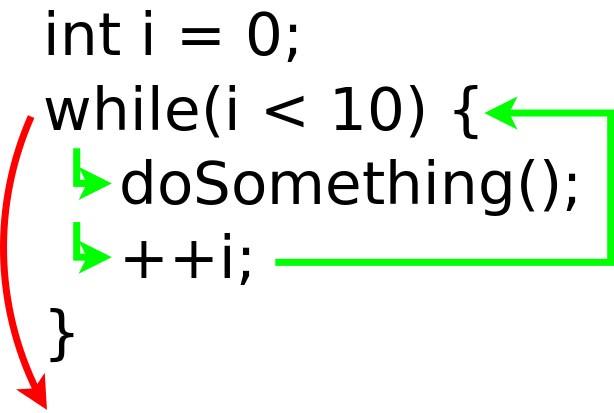
\includegraphics[width=0.75\textwidth]{img/while.png}
\end{frame}

\subsection{do while}
\begin{frame}{\subsecname}
  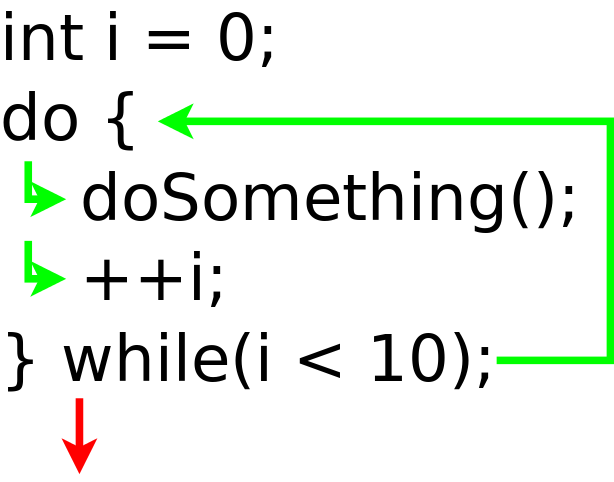
\includegraphics[width=0.75\textwidth]{img/dowhile.png}
\end{frame}

\subsection{for}
\begin{frame}{\subsecname}
  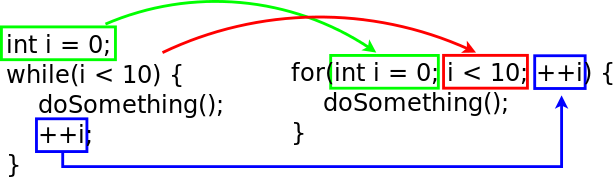
\includegraphics[width=\textwidth]{img/forwhile.png}
\end{frame}

\begin{frame}{\subsecname}
  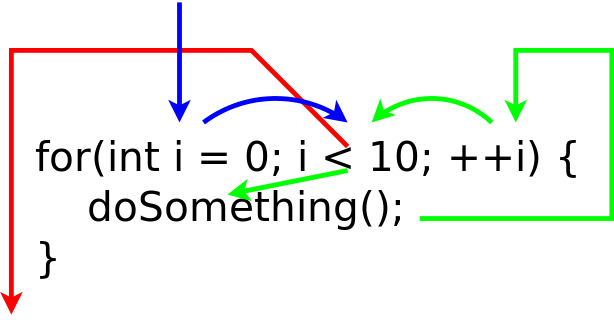
\includegraphics[width=\textwidth]{img/for.png}
\end{frame}

\section{Programmieren}
\begin{frame}{\secname}
  \begin{lstlsiting}
    goto eclipse;
  \end{lstlsiting}
\end{frame}

\end{document}
